\documentclass[12pt]{article}  % [12pt] option for the benefit of aging markers
\usepackage{amssymb,amsthm}    % amssymb package contains more mathematical symbols
\usepackage{graphicx}          % graphicx package enables you to paste in graphics
\usepackage[capposition=top]{floatrow}
\usepackage{setspace}
\usepackage{float}
\usepackage[backend=bibtex,sorting=nyt,firstinits=true]{biblatex}
\usepackage{hyperref}
\usepackage{longtable}
\usepackage{wrapfig}
\usepackage[titletoc,title]{appendix}
\usepackage{pdfpages}
\usepackage{color, colortbl}
\usepackage{tikz}
\usepackage{pgf-pie}
\usepackage{pgfplots}

\usepackage{lipsum}
\usepackage[margin=2cm]{geometry}

\definecolor{Gray}{gray}{0.9}


\addbibresource{references.bib}
\newcommand{\rid}[1]{\centering #1-\ifnum\value{requirement}<10 0\fi\arabic{requirement} \stepcounter{requirement}}






%PHP Code Listings Code %

\usepackage{listings,xcolor}
%\usepackage{inconsolata}

\definecolor{dkgreen}{rgb}{0,.6,0}
\definecolor{dkblue}{rgb}{0,0,.6}
\definecolor{dkyellow}{cmyk}{0,0,.8,.3}
\definecolor{backcolour}{rgb}{0.95,0.95,0.92}

\lstset{
  language        = php,
  basicstyle      = \small\ttfamily,
  keywordstyle    = \color{dkblue},
  stringstyle     = \color{red},
  identifierstyle = \color{dkgreen},
  commentstyle    = \color{gray},
  emph            =[1]{php},
  emphstyle       =[1]\color{black},
  emph            =[2]{if,and,or,else},
  emphstyle       =[2]\color{dkyellow},
  numbers = left,
  backgroundcolor=\color{backcolour},
  frame = single, 
  framexleftmargin=1.5em,
  xleftmargin=2em,
  breaklines= true
  }
  
%End of PHP Code Listings Code %



%%%%%%%%%%%%%%%%%%%%%%%%%%%%%%%%%%%%%%%%%
%										%
%     			Title					%
%										%
%%%%%%%%%%%%%%%%%%%%%%%%%%%%%%%%%%%%%%%%%
\title{Digital Lab Marking System \\~\\  \large{Heriot-Watt University} \\~\\ Deliverable 1: Final Year Dissertation \\~\\ MEng Software Engineering}
\author{Lewis Francis McNeill\\
supervised by
Peter J King}

\begin{document}
\maketitle
\pagenumbering{gobble}



%%%%%%%%%%%%%%%%%%%%%%%%%%%%%%%%%%%%%%%%%
%										%
%     		    Declaration				%
%										%
%%%%%%%%%%%%%%%%%%%%%%%%%%%%%%%%%%%%%%%%%
\newpage
\setcounter{page}{1}
\pagenumbering{roman}
\doublespacing
\textbf{\Large{Declaration}} \\[2em]
I, Lewis Francis McNeill, confirm that this work submitted for assessment is my own and is expressed in my own words. Any references, made within it, of the works of other authors in any way (e.g., ideas, equations, figures, text, tables, programs) are properly acknowledged at any point of their use. A list of the references employed is included.
\\
\\
Signed: Lewis McNeill
\\
Date: \today


%%%%%%%%%%%%%%%%%%%%%%%%%%%%%%%%%%%%%%%%%
%										%
%     		    Abstract				%
%										%
%%%%%%%%%%%%%%%%%%%%%%%%%%%%%%%%%%%%%%%%%
\newpage               
\begin{abstract}
\noindent
The aim of this dissertation project is to replace the current system for the marking of computer labs with a new digital system. This will enable lecturers to create a marking scheme online. Lab helpers will select the student they are marking and the marking scheme will then be loaded, marks will be entered and then made immediately available to both student and lecturers to view. It will also provide useful statistics for both student and lecturers.
\end{abstract}
\newpage 

\tableofcontents
\newpage
\listoffigures
\listoftables


%%%%%%%%%%%%%%%%%%%%%%%%%%%%%%%%%%%%%%%%%
%										%
%     		Introduction				%
%										%
%%%%%%%%%%%%%%%%%%%%%%%%%%%%%%%%%%%%%%%%%
\newpage   
\setcounter{page}{1}
\pagenumbering{arabic}
\section{Introduction}

The current system for marking of computing science labs is to use multiple lab helpers, each given a list of students and the marking scheme for them. Generally marking schemes are a selection of tasks students must have completed and lab helpers tick them off when this has been achieved. The biggest problem with this part of the marking is the length of time it takes lab helpers to locate the students on the list. This causes frustration with increased waiting times for students.  Multiple other issues  can also  arise from this: students can be marked by two helpers and obtain different grades from both; the lab helper omits to  tick off a completed task; they assign  marks for the wrong student on the sheet or simply they misplace the actual marking sheet.

After the lab helpers have completed their marking, the sheets are provided to the lecturer who collates them together into one spreadsheet to calculate marks. After that it is entered it into vision. This too can cause its own set of problems-the chances of transcription errors are increased as it is possible for the lecturer to misread marks when they are transferring them across. The lecturer may not enter the marks immediately into the spreadsheet increasing the chance that a marking sheet goes missing, and finally this system means that students are having to wait even longer to receive their results.

The objective is to develop a system that will reduce and hopefully eliminate the problems of the current system. Along with this, it should hopefully reduce the amount of time taken to mark students’ work and therefore speed up labs in general. It should also enable students to see their grades immediately, allow lecturer to see the result of the assignments as they are being marked and make marking quicker for lab helpers.




\newpage
\section{Aims and Objectives}
\subsection{Aim}
The aim of this dissertation is to design and implement a system for the digital marking and analysis of computer labs and to help improve the speed at which they are marked. The system will also provide useful statistics for both lecturers and students.

\subsection{Objectives}
\label{section:object}
\begin{itemize}
\item Simplify the way that labs marks are currently processed.
\item Allow lecturers to create marking schemes on-line that lab helpers can access. 
\item Lab helpers can mark students in labs using marking schemes.
\item Lab helpers able  to mark labs using an on-line application.
\item Allow students to see the mark they achieved from the lab instantly.
\item Provide useful statistics and graphs for lecturers and students.
\item Provide different views for student, lab helpers and lecturer.
\end{itemize}



\subsection{Scope}





%%%%%%%%%%%%%%%%%%%%%%%%%%%%%%%%%%%%%%%%%
%										%
%     	   Literature Review			%
%										%
%%%%%%%%%%%%%%%%%%%%%%%%%%%%%%%%%%%%%%%%%
\newpage
\section{Background Information}
This section contains the summaries of literature relating to the topic and should help to create a context for the development of a digital marking system. It will cover what marking systems that are currently being used, what current digital marking systems actually exist and why they are an improvement. Along with this it will also cover how to control what users are allowed to see, as well as explaining systems for creation of custom website forms, and finally it will cover the graphical displaying of statistics. 


\subsection{Web Applications}

\subsection{HTML}
Hypertext Markup Language (HTML) is a markup language that is used to create the structure of a website through the use of elements which are represents by tags (\textless html\textgreater, \textless href\textgreater, \textless a\textgreater). 

\subsection{Cascading Style Sheets}
Cascading Style sheets (CSS) is used to change the properties of elements created using HTML through the changing of these properties developers can change the look and response of a website. 

 

Then it comes to websites there can be multiple different Cascading Style Sheets being used.  

As part of this project I will be using CSS 3 which at time of write (2017) is the currently agreed standard \cite{noauthor_css_nodate}.


\subsection{Java-script}

\subsection{PHP}
\label{sec:php}

PHP stands for Hypertext Preprocessor and is an open source scripting language first developed in 1994 \cite{noauthor_php:_nodate} which can be embedded into HTML. Unlike HTML which is sent to the user and process by their computer, PHP scripts are instead processed by the website server. Once it has been processed HTML is generated and sent to the user. 

It currently has two major version which are version 5.x and 7.x


For this project I will be using version 5.6.25 as version 5 is still the most common version of PHP and allow for easy installation of the lab marking system into the universities server.



\subsection{Marking Systems}

\subsubsection{Lecturer Based}
The way lecturer based marking works is that students complete their assignment, the lecturer or tutor marks it and provides result in a timely manner with useful feedback which can be majorly important in helping students improve their skills  \cite{tang_investigating_2011}.

The advantage of this style of marking is that students can obtain useful feedback from their lecturer that can help improve their learning.  An article study \cite{higgins_conscientious_2002} found that of the students, when surveyed 82\% agreed to the question "I pay close attention to the comments I get" in response to assignment feedback.

A downside to this style of marking is that as the number of students increases on courses the amount of time required to mark assignments consequently takes longer and in some cases this can actually cause marked assessments to be scrapped completely due to the amount of time taken to give feedback to students \cite{brown_assessment_1999}.


\subsubsection{Peer Based}
To cope with increasing class sizes some courses are beginning to move towards peer marking. Peer marking system works by having students assess each other and in some cases  the students produced their own marking criteria \cite{orsmond_use_2000}.

This style allows  students to gain experience in evaluating other people's work, which some graduates feel is a necessary skill to possess. \cite{langan_insights_nodate}. Peer marking also deals with increasing amounts of students very well- this is because as the number of students increases the number of markers also increases!

Peer marking however has its own set of problems - for example, "Students may have a less well developed sense of the criteria compared to the lecturer which could lead to a lack of reliability of student marking." \cite{orsmond_use_2000}.



\subsection{Digital Marking Systems}

\subsubsection{Reasons for Digital Marking}
Digital marking systems are designed to mirror the current paper based marking systems but with the advantage of the electronic environment \cite{heinrich_online_2003}. These systems help to reduce the increasing workload caused by more and more students taking courses. Along with this it also allows administrative tasks associated with coursework to be automated enabling more time for other tasks.\cite{joy_effective_1998}.

For students digital marking is great as it allows for quick feedback as the assessor is able provide students feedback immediately after they have written it up, instead of having to wait for a class to receive it. In one study\cite{dahl_turnitin_2007} they found that 78\% of students would like get their feedback  electronically .

According to the highlighted article \cite{derby_duplication_2008} plagiarism is on the rise amongst student. This is where digital marking can help to reduce plagiarism as the programme can  do what a human marker cannot. They can compare a submission thousands of documents and judge if a person has plagiarised. They can also help to show patterns in assignments and marks that normally might go unnoticed.


\newpage
\subsubsection{TurnItIn}
There currently exists an on-line electronic plagiarism system called TurnItIn, \cite{noauthor_turnitin_nodate} currently being used by many universities around the world. It allows students to upload their essay assignments online. It then checks for plagiarism in the document by searching the internet and using a large database of documents. After it processes the document it assigns a plagiarism percentage and highlights any areas that were plagiarised. Lecturers can then login and view all the submitted documents and mark them .\\
Current research highlighted \cite{dahl_turnitin_2007} conducted a questionnaire and found that students felt that the system was easy to use and more convenient than having to provide paper copies. It also found that 50\% of students strongly agreed and 33.3\% just agreed that they preferred to have their grade shown online rather than have a cover sheet.

\subsubsection{BOSS System}
The BOSS system  was developed at the University of Warwick to help deal with their problem of having too many students for the number of staff and yet wanting students to have accurate and quickly available feedback \cite{joy_boss_2005}.
It is an electronic submission and assessment system created to allow computing science students to submit their programming assignments and have them tested and marked online \cite{joy_effective_1998}. The system is not designed to remove human markers completely, instead simply "assist the instructor in achieving a quicker, more accurate and more consistent assessment of programming assignment"\cite{joy_boss_2005}.

When a file is first submitted it is run through a plagiarism check to make sure that the submission is actually the student’s own work. It also checks that the submission passes pre-set tests to make sure it works. After this it goes into the evaluations stage, since evaluation attributes of code can be very subjective what the second step does is generate metrics about the submitted program. Some of these metric are a number of comments and percentage of methods declared \cite{joy_effective_1998}, which will help human markers evaluate the submission quicker.



\subsection{User Access Views}

\subsubsection{Social Media}
Controlling the view that users have, based on their access level, is common practice. Social media websites for instance allow users to limit what others  can see, through the use of a privacy setting \cite{tufekci_can_2008}. This means that another user's view is determined by the access level they are given for example, a user that is a friend will have a higher access and be allowed to see their whole feed, while an other users access may only allow them see the profile name.

\subsubsection{Database Controlled Access}
The patent highlighted \cite{noauthor_system_1997}, describes a system of limiting user web page access through the use of relation databases. The system would work by using two databases; one would hold a list of all the url's and associated access level, while the second database would hold all the user id's along with their assigned access level. When a user requests a webpage, the access level for that webpage and the user are looked up. If the users do not have the appropriate access they are denied permission to load the page and depending on implementation may be redirected to another webpage.
The design of this system is well suited for scalability since no matter how large the two datasets are only one piece of data is need from each database to confirm whether a user is allowed access.


\subsection{Custom Input Forms}

\subsubsection{SurveyMonkey}
Survey Monkey \cite{finley_surveymonkey_1999} is an example of custom web forms being created by users. Founded by Ryan Finley in 1999 Survey Monkey enables users to create their own surveys and easily distribute them. It builds the surveys by letting the user select the contents of the question and what the response type will be: The user can also decide if the responses are completely anonymous by default and the participants ip address is stored when they complete the survey. The users can continue to add as many questions as they would like, even after the survey is initially created. After designing the survey the user chooses how they would like to have their survey distributed. The available options that can be selected are a web link, social media, email or embeddable on a website \cite{waclawski_how_2012} .

When participants complete the survey their results are immediately stored and the results of the survey are visible to the user by login into their account on surveymonkey. They can choose to look at the responses individually or look at metrics about how participants responded.


\subsubsection{Customizing Forms In Electronic Mail Systems}
\noindent
A patent \cite{noauthor_customizing_2006} describes a process for user-customisable forms in an e-mail system where the administrator selects custom field types and behaviours.  For example current e-mail forms have

\begin{wrapfigure}[7]{r}{0.5\textwidth}
\vspace*{-\baselineskip}
\begin{figure}[H]
\includegraphics[width=0.7\textwidth]{images/emailform.png}
	\caption{Example Form (Patent \cite{noauthor_customizing_2006})}
	\label{fig:emailform}
\end{figure}
\end{wrapfigure}

\noindent
a field for address, subject and one for the the actual message to be sent. While an example of what the patent is suggesting can be seen in figure \ref{fig:emailform}, it shows the adding of additional fields allowing for wide variety of form to be created and not limit the  users to use the few forms that are precreated.\\
This increased flexibility in email forms would allow for easier  interpretation of messages, making responding or providing information via email a lot simpler and quicker.


\subsection{Development Tools}
%TODO%



\subsubsection{jQuery}
jQuery is a JavaScript library that is designed to improve and enrich the 



\subsubsection{Twitter Bootstrap}
Twitter bootstrap is a front-end framework \cite{noauthor_bootstrap_nodate} designed to help developers create dynamical responsive websites quickly and easily. It provides pre-created cascadding style sheets (CSS)

\subsubsection{PHP Unit}

PHP Unit is a testing framework for PHP. It is designed to allow the easy creation of automated tests in the form of unit tests \cite{bergmann2005phpunit}. 

The most recent stable version is PHPUnit 6.0, this version is only compatible with PHP version 7 and was released on the 8th of Feburary 2017. Since I am using PHP 5.6.25 as stated earlier in Section \ref{sec:php} I can not use this most recent version and will instead be be using an older stable version 5.7 which supports PHP version 5.6, 7.0 and 7.1. That version was released on 2nd December 2016.



\subsubsection{D3}
D3 \cite{bostock_d3.js_nodate} is a javascript library, which was designed for the creation of interactive visualisations of data and was first developed in 2011. D3 uses precreated Javascript functions to create scalable vector graphics (SVG's) which are embedded into the HTML of websites."SVG is a language for describing two-dimensional graphics in XML"\cite{ferraiolo_scalable_2000} and can have displays changed  using Cascading Style Sheet (CSS).  \\
Data-sets can also be bound to an SVG allowing for a visual way to interpret the data-set, and as the data-set changes the SVG will be changed allowing for a dynamic display.



\subsubsection{CakePHP}
CakePHP is an open source framework for php, it is developed to help with rapid development of web application and make them simpler,fast and less complex to build \cite{noauthor_cakephp_nodate}. It allows the development of well structured and robust web applications \cite{plekhanova_evaluating_2009}, and its latest version is version 3.3 called "Red Velvet" it can be downloaded from (https://cakephp.org/).

The usefulness of the framework come in the form of its predefined functions, it allows for more secure code, since you cannot accidental forget to escape character from input as the functions do this anyway. Cakephp helps to improve the maintainability of systems as it is easy to understand with plenty of comments.

A downside to cakephp is its testability, compared to other web frameworks it lacks in testing tools and does not contain a testing environment \cite{plekhanova_evaluating_2009}.


%%%%%%%%%%%%%%%%%%%%%%%%%%%%%%%%%%%%%%%%%
%										%
%     		 Requirements				%
%										%
%%%%%%%%%%%%%%%%%%%%%%%%%%%%%%%%%%%%%%%%%
\newpage
\section{Requirements}
\label{section:require}
\newcounter{requirement} \stepcounter{requirement}


\subsection{Requirements Analysis}
To help find out the requirements of the lab marking system I preformed a requirements analysis questionnaire(Full questionnaire in Appendix \ref{app:requirements}), the questionnaire was given to lab helpers and lecturers to help understand what they would both want out of the system. 

The results of the requirements analysis was used to develop and refine the the list of requirements displayed, functional requirements can be found in section \ref{sec:func} and non-functional requirements in section \ref{sec:non-func}.



\subsection{Requirements}
\label{sec:requirements}
Requirements for the system are each given an idea depending on the type of requirement: FR for functional requirements and NFR for non-functional requirements.

Along with this, each requirement has a description stating what the requirement is and a  priority is assigned using the MoSCoW prioritization method discussed in the next section (\ref{sec:moscow}).


\subsubsection{MoSCow Prioritisation}
\label{sec:moscow}

MoSCow Prioritisation \cite{noauthor_moscow_2015} was designed to be used in project that utilise agile development and have a fixed time limit in which to be completed. The way that it works is that all the requirements of the project are prioritised into four categories, these are:

\begin{itemize}

\item \textbf{Must:} This category of requirements make up the "\underline{M}inimum \underline{U}sable \underline{S}ubse\underline{T}" of requirements that the project must implement to be successfully delivered.

\item \textbf{Should:} This category contains requirements that are not vital to the delivery of the project, but their absence can effect the project overall. 

\item \textbf{Could:} This category contains requirements that are wanted in the system but are less important than the "should" priority. Reasons that a requirement would become a could instead of a should is if the amount of time take to implement the requirement outweighs the effect if will have on project.   

\item \textbf{Won't:} This category contains all the requirements that will not be implemented in the delivered project, but could be implemented in later development.
\end{itemize}

\noindent For this project I will be attempting to implementing all of the must priority functional and nonfunctional requirements, I will also try and implement all of the should requirements. Finally I will implement as many of the could priority requirements that I can starting with ones that best improve the system.


\def\arraystretch{1.5}
\subsubsection{Functional Requirements} \label{sec:func}

Functional requirements also include an access column which defines what users should be able to use. Some items are restricted to lecturers as some requirements should only be be usable by lecturers and lab-helpers and not by students. The table is sorted first by access level starting with widest allowed access then sorted in access order 1 - 4, it is secondly sorted by priority.

The access levels are: 1-Admin, 2-Lecturers, 3-Lab Helpers and 4-Students

\begin{spacing}{1.5}
\begin{longtable}{|p{0.09\linewidth}|p{0.6\linewidth}|p{0.1\linewidth}|
p{0.1\linewidth}|}
\caption{Functional User Requirements} \label{table:funct-user} \\ \hline
\textbf{ID} & \textbf{Requirement} & \textbf{Access} & \textbf{Priority}\\
\hline \hline

\rowcolor{Gray} \rid{FR} & Login to view system & 1,2,3,4 & Must\\ \hline
\rid{FR} &  Accounts created for them & 1,2,3,4 & Must\\ \hline
\rid{FR} &  Change password & 1,2,3,4 & Must\\ \hline
\rid{FR} &  Login using university ID & 1,2,3,4 & Won't\\ \hline
\rid{FR} &  Logout & 1,2,3,4 & Must \\ \hline

\rid{FR} &  Remove students from courses & 1, 2 & Must\\ \hline
\rid{FR} &  Update student accounts & 1,3 & Won't \\ \hline

\rid{FR} &  Look up students in lab & 2,3 & Must\\ \hline
\rid{FR} &  Select students from lab list & 2,3 & Must\\ \hline
\rid{FR} &  Leave comments about students & 2,3 & Must\\ \hline
\rid{SR} &  Save marks & 2,3 & Must\\ \hline
\rid{SR} &  Update marks & 2,3 & Must\\ \hline
\rid{SR} &  Delete marks & 2,3 & Must\\ \hline
\rid{FR} &  Search for student by name & 2,3 & Medium\\ \hline
\rid{FR} &  Mark student even if they are not in the system & 2,3 & Could \\ \hline

\rid{FR} &  Assign students to courses & 1 & Should\\ \hline
\rid{FR} &  Assign lectures to courses & 1 & Should\\ \hline

\rid{FR} &  Create marking schemes & 2 & Must\\ \hline
\rid{FR} &  Display generated stats & 2 & Must\\ \hline
\rid{FR} &  See submitted marks & 2 & Must\\ \hline
\rid{FR} &  Generate end of year spread sheets & 2 & Should\\ \hline
\rid{FR} &  Editing of students in class & 2 & Should\\ \hline
\rid{FR} &  Create peer marking scheme & 2 & Could\\ \hline
\rid{FR} &  Look at students stats & 2 & Should\\ \hline
\rid{FR} &  Set what parts of the marking scheme students can see & 2 & Could\\ \hline
\rid{FR} &  Update marking scheme & 2 & Should \\ \hline
\rid{FR} &  Delete marking schemes & 2 & Should\\ \hline
\rid{FR} &  Able to assign students to set labs & 2 & Won't \\ \hline
\rid{FR} &  Set penalties for late marking & 2 & Won't \\ \hline
\rid{FR} &  Able to export to vision & 2 & Won't\\ \hline

\rid{FR} &  Access Marking Scheme & 3 & Must\\ \hline
\rid{FR} &  Enter selected students mark & 3 & Must\\ \hline
\rid{FR} &  Submit student mark & 3 & Must\\ \hline
\rid{FR} &  Select the lab they are helping in & 3 & Must\\ \hline

\rid{FR} &  See current mark & 4 & Must\\ \hline

\rid{FR} & Show different displays depending on access level & & Must\\ \hline
\rid{FR} & Load students current lab mark scheme & & Must\\ \hline
\rid{FR} & Apply penalty for late lab completion & & Could\\ \hline
\rid{FR} & Create a set of useful stats based on lab & & Must\\ \hline
\rid{FR} & Store what class student belong too & & Must\\ \hline
\rid{FR} & List of all students in class & & Must\\ \hline

\end{longtable}
\end{spacing}
\setcounter{requirement}{1}


\newpage
\subsubsection{Non-Functional Requirements} \label{sec:non-func}

Table \ref{table:non-func} lists all the non-functional requirements for the development of the system, they are ranked in order of priority.

\begin{spacing}{1.5}
\begin{longtable}{|p{0.1\linewidth}|p{0.7\linewidth}|p{0.1\linewidth}|}
\caption{Non-Function Requirements} \label{table:non-func}\\
\hline
\textbf{ID} & \textbf{Requirement} & \textbf{Priority}\\
\hline \hline


\rid{NFR} & All person data encrypted & Must\\ \hline
\rid{NFR} & Update stats as marks are entered & Must\\ \hline
\rid{NFR} & Take less than 2 seconds to generate stats  & Must\\ \hline
\rid{NFR} & PHP Should use prepared statements & Must\\ \hline
\rid{NFR} & Website dynamically designed & Must\\ \hline
\rid{NFR} & HTML, CSS and Javascript should be validated & Must\\ \hline
\rid{NFR} & Should make sure inputs are valid & Must\\ \hline
\rid{NFR} & Should prevent SQL Injection & Must\\ \hline


\rid{NFR} & Function on a wide variety of smart phones and tablets & Should\\ \hline
\rid{NFR} & Handle a large number of users without any faults & Should\\ \hline
\rid{NFR} & Check passwords contain alphanumerics and have a minimum and maximum length  & Should\\ \hline
\rid{NFR} & Auto save marks as they are entered & Could\\ \hline
\rid{NFR} & Auto record what lab help marked what student & Could\\ \hline
\rid{NFR} & List all students that did not attend the lab & Could\\ \hline
\rid{NFR} & Track how long it takes to mark a student & Could \\ \hline


\rid{NFR} & Disability options (Increase text size, colour layout) & Won't\\ \hline
\rid{NFR} & Readable by screen readers & Won't\\ \hline
\rid{NFR} & Take less than 2 second to load student marking scheme & Won't\\ \hline
\rid{NFR} & Group marked people & Won't \\ \hline
\rid{NFR} & Retrieve student images from university system & Won't\\ \hline
\rid{NFR} & Backup database regularly & Won't\\ \hline


\end{longtable}
\end{spacing}
\setcounter{requirement}{1}


%%%%%%%%%%%%%%%%%%%%%%%%%%%%%%%%%%%%%%%%%
%										%
%     		     Design 				%
%										%
%%%%%%%%%%%%%%%%%%%%%%%%%%%%%%%%%%%%%%%%%
\newpage
\section{Design}
This sections is to explain all the design decision take in developing the marking system using sketches, models and diagrams and thus assist in the understanding of how the system works as a whole. The design aspect that are cover are: the user interface, database design and the main functionality required to make the system work. 

\subsection{User Interface Design}
For the system to be useful the user interface must be easy to use and understand, along with this it will have to be functional on mobile devices as well. To achieve this I have developed mock-ups for main web pages required to make the system work, including a design for desktop and mobile. 

\subsubsection{Lab Results}
For the system to be useful students and lecturers both need to be able to see the results of a lab. For this apart of the application there needs to be two different views depending on the type of person signed in. This is because students need to only see their own results, while lecturers need to be able to select students and see their mark. To help develop the two different displays I have created a design for how lab results should displayed for students (figure [lfm]), and another one for lecturers (figure [lfm]). 


\subsubsection{Lab Marking}
The lab marking page is designed to allow lab helpers and lecturers to easily select which course and lab they are marking, and then be provided with list of students who can be marked.

I expect this page to be used more on mobile devices, since it easier carry a mobile device than log-in to each computer this is reflected in the mobile design shown in figures([lfm]).


\subsubsection{Lab Creation}
The "Lab Creation" page will be very important for lecturers as they will have to use to to create all of their labs. Given that courses tend to have a fair number of labs it is likely lecturers will have to use this part of the system fairly often, therefore the process for creating a lab should be fairly simple. These idea are reflected in the designs shown in figures([lfm]).


\noindent In the desktop design the side bar contents have been swapped for buttons one for each of the different types of question that a lab can have. Along with this the main content area has a drop down menu to allow lecturers to select the course they would like to create the lab for, and next too that a input box to allow them to provide the labs name.

The questions themselves are designed with simplicity in mind, lecturers select what type of question they want by clicking it on the left hand side and a new question tile appears in the main content area. The question tiles state what type of question they are what question number they will be and have remove button. To add the question text lecturers just fill out the question input box, and depending on the type of question select how many marks it is worth from the drop down menu. 

The mobile version is the same but with the side bar being moved to the top and the question type buttons being underneath the navigation bar.



\subsubsection{Lab Manager}
The "Lab Manager" page is what lecturers will use to control labs that they have already created. Functionality available from here include: the ability to delete a lab, edit a lab, set whether lab-helpers are able to mark a lab and being able to export all the results for a selected lab. The desktop and mobile designs can be seen in the figure below ([lfm]). 



\newpage
\subsection{Database Design}
\label{sec:design-db}
For the system to work there will need to be database that stores students, labs, and marks received. The database schema I will be using for this system is shown in figure(\ref{fig:dbschema}) below.

\begin{figure}[H]
    \fbox{
    \includegraphics[width=1\textwidth]{images/design/DB_Diagram.png}}
	\caption{Database Schema}
	\label{fig:dbschema}
\end{figure}

\noindent The database can be broken down into three section a shown in figure(\ref{fig:dbsections}). The first sections ([lfm]) is designed for storing all the users of the database, it is designed to be easily changed to allow for easy integration into already existing databases. As long as users have unique ID's the rest of the database will be able to function with no changes being required.

Section two ([lfm]) is designed to storage information relating to users and courses. The Students on Courses table stores what students are on what course, The lab helpers table stores what courses a lab-helper is helping and finally the Course Lecturer tables stores what courses lectures are teaching.

The third section ([lfm]) is entirely to do with the storage of information relating labs.

\begin{figure}[H]
    \centering
    \includegraphics[width=0.5\textwidth]{images/design/DB_Sections.png}
    \caption{Database Sections}
    \label{fig:dbsections}
\end{figure}

\subsection{Functionality Design}
%TODO%







%%%%%%%%%%%%%%%%%%%%%%%%%%%%%%%%%%%%%%%%%
%										%
%     		 Implementation				%
%										%
%%%%%%%%%%%%%%%%%%%%%%%%%%%%%%%%%%%%%%%%%
\newpage
\section{Implementation}
This section documents and explains how the lab marking system was developed and the key functionality works. 

This is done through the use of screen shots showing the functionality, code snippets with explanations on what it does and how.   

\subsection{Database}

The database schema discuss in the design section (\ref{sec:design-db}) was converted into a relational database using mysql. Figure \ref{fig:implement-db} displayed below shows the database structure and the lines between tables shows their relations. There a no major changes from the original design, the only difference that occured during implementation was that some of the attribute names were changed different.  

\begin{figure}[H]
    \centering
    \includegraphics[width=1\textwidth]{images/implementation/database.png}
    \caption{Implemented Database Schema}
    \label{fig:implement-db}
\end{figure}

\subsection{PHP Class Structure}

All the PHP developed as part of this project was built on a class structure, each class contains the functionality for a part of the system. Many of the classes inherit functions from other classes and the relationship diagram can be seen in figure([lfm]). 

When it came to the creation of classes and their inheritance there are limitation created by PHP. In PHP class are only able to extend one other class, the only way to inherit multiple classes is to create an instance of it instead. This is usually done in the construct so that the class may be accessed through a private variable. 


In my classes I do a combination of constructor declared instances, and instances declared in functions






\subsection{Background Functionality}

This section is for the classes and functionality that are not dedicated to one part of the system, but are used by multiple different classes to provided key functionality for them to work.  

\subsubsection{Database Connection}

The ConnectDB class is designed to create a connection to the database and allow other classes to retrieve information through the connection. The class also has a secondary function of checking if a session has been started and if not starting one, this is to allow access to sessions that may be needed for querying the databse. The full code listing can be seen below (\ref{lst:connect-db}).

\singlespacing
\begin{lstlisting}[basicstyle=\linespread{0.8}, caption= Database Connection Class, label = lst:connect-db]
class ConnectDB
{
    public $link;

    function __construct()
    {
        $this->link = mysqli_connect('host', 'username','password');
        if(!$this->link) {
            die('Could not connect to MySQL: ' . mysqli_connect_error());
        }

        mysqli_select_db($this->link,"lab-marker"); //Selects the Database

        if (session_status() == PHP_SESSION_NONE)
            session_start();
    }
}
\end{lstlisting}
\doublespacing

\noindent The way that the class works is, it contains one public variable called \$link; when the class is initilised the constructor function called. The constructor makes a mysqli connection using the provided host, username and password details, it then sets the \$link variable to the result of the connection. After this it check if the connection was successful, if it is not then a die command is thrown and an error message is shown. If it is a successful connect then is selects the "lab-maker" database. Checks if a session is already run, and starts one if it is not.

\subsubsection{Security}
\label{sec:security}





\subsection{Lab Creator}
The design of the lab creation page can be seen in figure(\ref{fig:lab-creator}) is almost identical to what its initial design showed. 

\begin{figure}[H]
    \centering
    \includegraphics[width=0.8\textwidth]{images/implementation/lab-creator-1-page.png}
    \caption{Lab Creation Page}
    \label{fig:lab-creator}
\end{figure}

\subsection{Marking Labs}
%TODO%

\subsection{Results Display}

The implementation of the results page required that it only show students their own marks. While lecturers were able to select a student and see his mark for a lab. They way that I went about doing this was by designing two similar web pages one for students (section \ref{sec:results-student}) and one with more functionality (section \ref{sec:results-lecturer}). Through the use of the security class discussed earlier (section \ref{sec:security}) when the user access the results page, their access level is check and then using PHP the respective layout is shown to them. Details on the ways that the displays are different and how they both function are discussed in the next two sections.



\subsubsection{Students View} \label{sec:results-student}

The design of the students results page remained similar to the initial design, however there was one major design change. Which was that in the initial design the results for each lab was shown straight way in there own table. This was replaced with lab summary area that when clicked expand to show the individual marks for the questions. This was done to help make the area nicer and make it easier to distinguish when one lab ended another one began. The students view of the results page can be seen in figure(\ref{fig:results-student}).


\begin{figure}[H]
    \centering
    \includegraphics[width=1\textwidth]{images/implementation/student-results-page.png}
    \caption{Students Results}
    \label{fig:results-student}
\end{figure}

\subsubsection{Lecturers View} \label{sec:results-lecturer}
%TODO%


\subsubsection{Expanding Table}




\subsection{Lab Management}
%TODO%

\subsection{Admin Panel}






%%%%%%%%%%%%%%%%%%%%%%%%%%%%%%%%%%%%%%%%%
%										%
%     		Testing & Evaluation		%
%										%
%%%%%%%%%%%%%%%%%%%%%%%%%%%%%%%%%%%%%%%%%
\newpage
\section{Testing}

This section states how the lab marking system was tested to assure the quality of the system and discover any unexpected bugs.

Testing of the system comprised of two stages, the first was the continues testing being done during development and the second being tests that were run when the system was completed to find any remaining bugs.


\subsection{Development Testing}
To help test functionality unit tests were created using the PHPUnit testing framework. Unit tests were developed for classes that provide key functionality to the lab marking system. 

\subsubsection{Security Class Tests}

The security class does all the checks on whether a user has the required access being requested. 

To test the security class but the hasAccessLevel and hasGreaterAccessThan functions were tested. Since the hasAccessLevel function checks if a users has equal to or greater access than that being requesting, all possible combinations of user access and requested access were tested and the expected outcomes compared to the actual result. The code for this can be seen in listing(\ref{lst:hasAccess-test})

\singlespacing
\begin{lstlisting}[basicstyle=\linespread{0.8}, caption= hasAccessLevel Test, label = lst:hasAccess-test]
public function testHasAccessLevel($user_access, $required_acess, $expected)
{
    if(session_status() == PHP_SESSION_NONE)
        session_start();
    $_SESSION["accesslevel"] = $this->security->getAccessValue($user_access);

    $result = $this->security->hasAccessLevel($required_acess);
    $this->assertEquals($expected, $result, $user_access . " and " . $required_acess . ": Failed");
}
\end{lstlisting}
\doublespacing



\subsection{Final Testing}

The final testing of the system came in two parts. The first part was the running of all the unit tests that were created to make sure all the different parts of the marking systems worked correctly, and could interact without causing any issues.

The second part of the final testing was to get users to test the system, and any bug found by users be recorded so that the source of the problem could be found. This testing was done as part of the usability case study 


\newpage
\section{Evaluation}

This section shows how I evaluated the lab marking system and help determine how successful I was at implementing the system, and what future improvements could be done to make the system more useful. 

\subsection{Usability Case Study}
The way the marking system was evaluated was through the use of a usability case study (UCS), participants for the study were students, lab helpers and lecturers. The case study provided a range of quantities and qualitative questions to help get the maximum amount of feedback about the lab marking system as possible. 


The usability case study consisted of four sections: student, lab helpers, lecturers and Mobile. Each section has specific tasks that participants were required to preform, they then evaluate how challenging the task was and provided comments about the design and any additional improvements that could be made. 

In the first three sections the participant signed into the system as that particular type of user (student, lab helper and lecture) 



(Appendix \ref{app:ucs})

\subsection{Feedback}

Due to the amount of time the case study required to be completed and the time at which I was trying to run it at, only twelve people took part in the in it. The breakdown of participants was: four lecturers, four lab-helpers and four students, thus providing an even sample for the types of users of the lab marking system.

The feedback that was obtain from the case study will be very useful in showing how successful the project was at creating a digital lab marking system, the feedback is broken up into two sections. The first sections is for the quantitative questions and the results that can be obtained from them. While the second question section will deal with all the qualitative questions and what can be gleaned from them. 



\subsubsection{Quantitative Questions}

This section is dealing with all the question in the usability case study that quantitative. In the case study there were two types of quantitative questions: scale questions and the other being  yes and no questions.

Scale questions were used to allow participants to evaluate how difficult a specific task was and ranged from one to five. One being very easy, three being challenging and five meaning the task was impossible to complete. 
The table below (table \ref{table:usability}) contains the mean, median, mode and overall difficulty of the task for each of the scale question in the case study. The difficulty is decided by rounding the mean value up or down.

\setlength\LTleft{0pt}
\setlength\LTright{0pt}


\begin{longtable}{@{\extracolsep{\fill}}|c|l|c|c|c|c|}
\caption{Usability Case Study: Scale Question Results} \label{table:usability} \\ \hline

\textbf{Question Number} & \textbf{Question} & \textbf{Mean} & \textbf{Median} & \textbf{Mode} & \textbf{Difficulty}\\ \hline

Q1.1 & Difficulty to find the students mark & 1.08 & 1 & 1 & Easy\\ \hline
Q1.3 & Difficulty to sign out & 1 & 1 & 1 & Easy \\ \hline

Q2.1 & Difficulty to mark a student & 1.92 & 2 & 2 & Quite Easy \\ \hline
Q2.2 & Difficulty to change student mark & 1.25 & 1 & 1 &  Easy \\ \hline

Q3.1 & Difficulty to view student marks as lecturer & 1.42 & 1 & 1 &  Easy \\ \hline
Q3.4 & Difficulty to make a new lab & 2.41 & 2.5 & 3 & Quite Easy \\ \hline
Q3.10 & Difficulty to export lab & 1.33 & 1 & 1 &  Easy \\ \hline
Q3.13 & Difficulty to delete lab & 1 & 1 & 1 &  Easy \\ \hline
Q3.16 & Difficulty to remove and add students & 1.5 & 1 & 1 &  Easy \\ \hline
Q3.18 & Difficulty to remove and add lab helpers & 1.08 & 1 & 1 & Easy \\ \hline

\end{longtable}

\noindent The graph below (figure \ref{graph:results}) displays how challenging all the participant found each of the questions, The y-axis represents the number of participants that thought at specific task was that difficulty. The x-axis represents each of the questions and are broken up into five bars each representing a difficulty. The left most bar represents easy and as the bars go to the right the difficulty increases until final one which represents impossible.  

\begin{figure}[H]
\caption{Bar Graph of Question Results}
\label{graph:results}
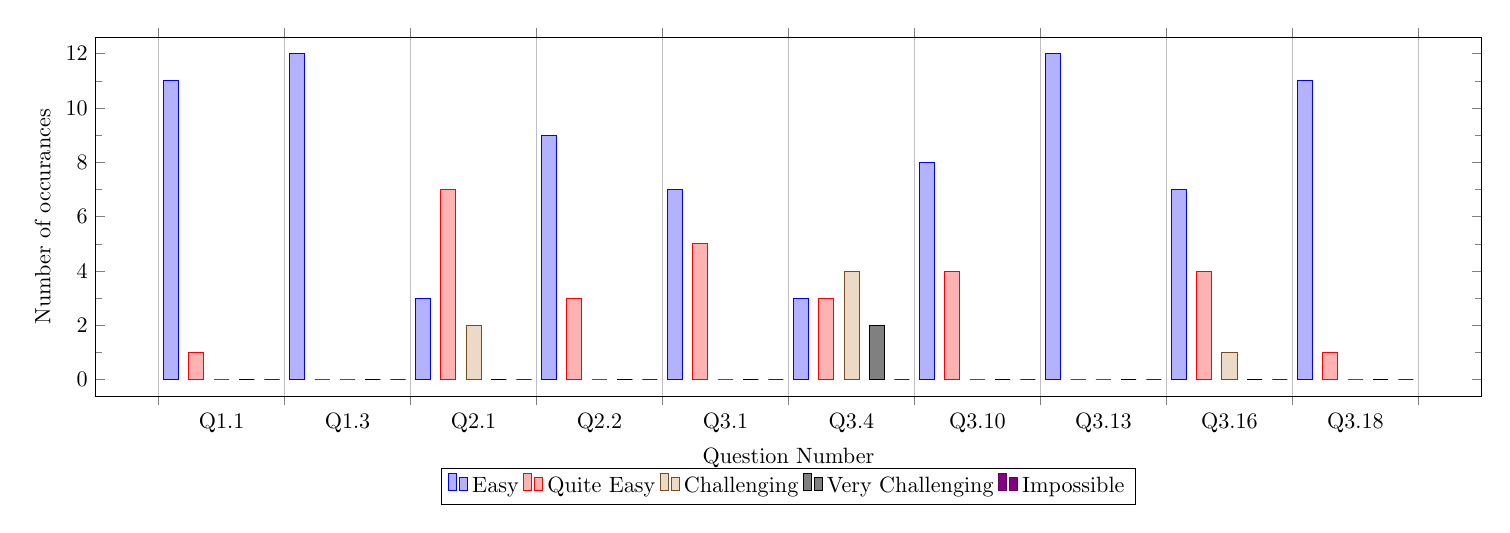
\begin{tikzpicture}[scale=0.8]
\begin{axis}[ybar interval, ymax=12, minor y tick num = 1, legend style={at={(0.5,-0.2)}, anchor=north,legend columns=-1}, bar width= 0.1cm, x=2cm, 	enlargelimits=0.05, ybar interval=0.6, xlabel= Question Number, ylabel= Number of occurances,symbolic x coords={Q1.1, Q1.3, Q2.1, Q2.2, Q3.1, Q3.4, Q3.10, Q3.13, Q3.16, Q3.18, None},xtick=data]


\addplot coordinates { (Q1.1, 11) (Q1.3,12) (Q2.1, 3) (Q2.2, 9) (Q3.1, 7) (Q3.4, 3) (Q3.10, 8) (Q3.13, 12) (Q3.16, 7) (Q3.18, 11) (None, 10)};

\addplot coordinates { (Q1.1, 1) (Q1.3,0) (Q2.1, 7) (Q2.2, 3) (Q3.1, 5) (Q3.4, 3) (Q3.10, 4) (Q3.13, 0) (Q3.16, 4) (Q3.18, 1) (None, 10)};

\addplot coordinates { (Q1.1, 0) (Q1.3,0) (Q2.1, 2) (Q2.2, 0) (Q3.1, 0) (Q3.4, 4) (Q3.10, 0) (Q3.13, 0) (Q3.16, 1) (Q3.18, 0) (None, 10)};

\addplot coordinates { (Q1.1, 0) (Q1.3,0) (Q2.1, 0) (Q2.2, 0) (Q3.1, 0) (Q3.4, 2) (Q3.10, 0) (Q3.13, 0) (Q3.16, 0) (Q3.18, 0)  (None, 0)};

\addplot coordinates { (Q1.1, 0) (Q1.3,0) (Q2.1, 0) (Q2.2, 0) (Q3.1, 0) (Q3.4, 0) (Q3.10, 0) (Q3.13, 0) (Q3.16, 0) (Q3.18, 0) (None, 0)};



\legend{Easy, Quite Easy, Challenging, Very Challenging, Impossible}
\end{axis}
\end{tikzpicture}
\end{figure}

%Overall easiness% 
The first thing that can be noticed is that overall the participants found the lab marking system to be fairly easy to use and understand. The two task that users found the hardest to do were mark students and create labs, which are the most complex part of the lab marking system . It would be expected that first time users of the system would find these are to understand at first. Tho it can be seen with the change student mark task that once the participant understood how to mark one student they could easy update their mark. 

%Difficulty of creating labs%
It can be seen thanks to graph shown in figure(\ref{graph:results} that many users found the creating of new labs to be a difficult task to complete. While watching participants  I noticed that many of them were confused on how questions were added to labs. 

%Simplicity of student section%
Question 1.1 tasked participants to sign in as a student and see what mark they were given. As the results of both the table(\ref{table:usability}) and the graph(\ref{graph:results}) all participants found this to be easy to do. This is great to see, as the lab marking system is meant to make it easier for students to find out their marks and this task has shown that process for a student finding there marks is very straight forward.


\subsubsection*{Yes/No Question}
Three of the questions in the usability study were yes and no questions. These questions were designed to see if users understood key parts of the lab marking system.

The first question was to check if participants understood what the different coloured buttons for students represented and 75\% did understand what they represented. 

\begin{figure}[H]
\caption{Q2.3: Know what the different student colours mean?}

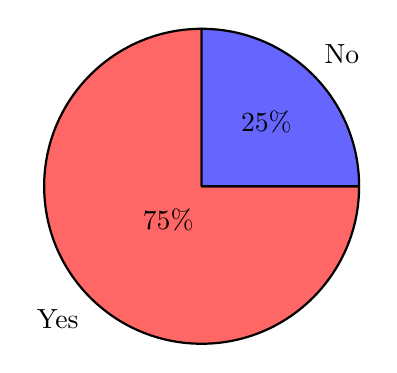
\begin{tikzpicture} 
    \pie[rotate=90,radius =2, color={red!60, blue!60}]{75/Yes, 25/No}
\end{tikzpicture}

\end{figure}



\begin{figure}[H]
\caption{Q3.6 Know what visible / not visible means?}

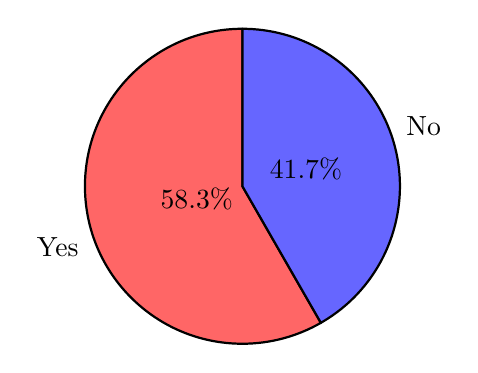
\begin{tikzpicture} 
    \pie[rotate=90,radius = 2, color={red!60, blue!60}]{58.3/Yes, 41.7/No}
\end{tikzpicture}

\end{figure}


\begin{figure}[H]
\caption{Q3.8: Did an alert appear}

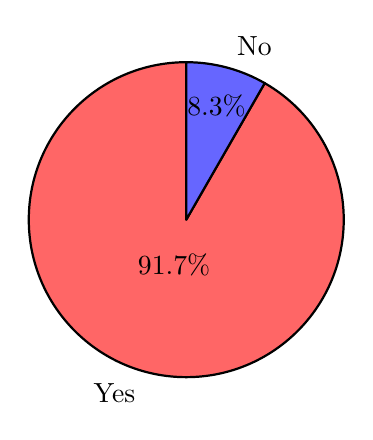
\begin{tikzpicture}
    \pie[rotate=90,radius =2, color={red!60, blue!60}]{91.7/Yes, 8.3/No}
\end{tikzpicture}

\end{figure}


\subsubsection{Qualitative Questions}

\subsection{Implementation Of Feedback}

Using the feedback obtained through the usability case study I have have implemented a few changes to the design of the lab marking system. This is to help improve the overall usefulness of the system and make certain parts of the system easier to understand and interact with. The improvements done to the system are listed below with description and comparison showing the lab marking system before and after the changes.   


%%%%%%%%%%%%%%%%%%%%%%%%%%%%%%%%%%%%%%%%%
%										%
%     	       Discussion				%
%										%
%%%%%%%%%%%%%%%%%%%%%%%%%%%%%%%%%%%%%%%%%
\newpage
\section{Discussion}
%TODO%

\subsection{Development}
%TODO%

\subsection{Limitations}
%TODO%

\subsection{Future Improvements}
The electronic marking system has many improvements that can be implemented some are requirements that I was not able to implement 

\subsection{Conclusion}
%TODO%









%%%%%%%%%%%%%%%%%%%%%%%%%%%%%%%%%%%%%%%%%
%										%
%     		Bibliography				%
%										%
%%%%%%%%%%%%%%%%%%%%%%%%%%%%%%%%%%%%%%%%%


\newpage
\printbibliography[heading=bibintoc]
\let\cleardoublepage\clearpage


%%%%%%%%%%%%%%%%%%%%%%%%%%%%%%%%%%%%%%%%%
%										%
%     		Appendices					%
%										%
%%%%%%%%%%%%%%%%%%%%%%%%%%%%%%%%%%%%%%%%%

\newpage
\begin{appendices}

\let\cleardoublepage\clearpage

% \chapter{Useability Case Study}
% \includepdf[pages={1}]{pdf/UseabilityCaseStudy.pdf}
% \section{Useability Case Study}
% \includepdf[scale=0.85, pages=-]{pdf/UseabilityCaseStudy.pdf}



%Requirements Analysis Document
% \includepdf[scale=0.9,clip,trim=0cm 0cm 0cm 2cm,pages={1},pagecommand={\section{Requirements Questionaire} \label{app:requirements}}]{pdf/RequirementsQuestionaire.pdf} 
% \includepdf[scale=0.9,clip,trim=0cm 0cm 0cm 2cm,pages={2-6},pagecommand={}]{pdf/RequirementsQuestionaire.pdf}


%Useability Case Study Document
% \includepdf[scale=0.9,clip,trim=0cm 0cm 0cm 2cm,pages={1},pagecommand={\section{Useability Case Study Questionaire} \label{app:ucs}}]{pdf/UseabilityCaseStudy.pdf} 
% \includepdf[scale=0.9,clip,trim=0cm 0cm 0cm 2cm,pages={2-8},pagecommand={}]{pdf/UseabilityCaseStudy.pdf}


\end{appendices}

\end{document}